\documentclass{report}
\usepackage{tikz}
\usepackage{subcaption}

\begin{document}
\begin{figure}
  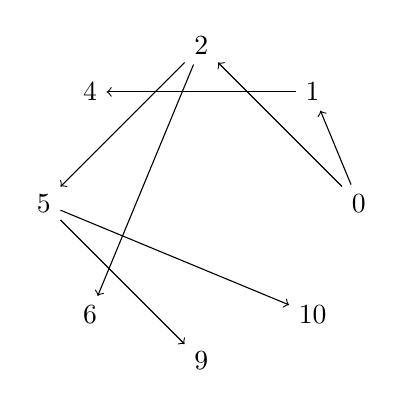
\begin{tikzpicture}
      \draw
        (0.0:2) node (0){0}
        (45.0:2) node (1){1}
        (90.0:2) node (2){2}
        (135.0:2) node (4){4}
        (180.0:2) node (5){5}
        (225.0:2) node (6){6}
        (270.0:2) node (9){9}
        (315.0:2) node (10){10};
      \begin{scope}[->]
        \draw (0) to (1);
        \draw (0) to (2);
        \draw (1) to (4);
        \draw (2) to (5);
        \draw (2) to (6);
        \draw (5) to (9);
        \draw (5) to (10);
      \end{scope}
    \end{tikzpicture}
  \caption{(.)* > (($A | $B)&$C)}
\end{figure}
\end{document}